\section{結論}
本研究ではKAGRAのサファイア鏡を吊るした低温懸架装置の一つであるETMXについて, 82 Kにおける特性を評価した. その結果, 先行研究で行われた測定と同様, 低温にするとフォトセンサの出力が1.8倍大きくなることが分かった. 一方で, MN段とIM段で用いられる12個のセンサの出力の範囲は, 82 Kにおいて平均値に対して32\%のばらつきがあることが新たに分かった. この結果はばらつきの範囲が50\%以下におさまる必要があるというKAGRAでの要求値を満たす. しかし, 冷却することによって出力にばらつきの範囲が徐々に大きくなるという結果も得られているため, 今後冷却が進んでも要求を満たすかどうかは, 注意して確認する必要がある. また, ETMXの機械的な共振周波数およびその伝達関数の低温にした際の変化量を測定した. その結果, 冷却に伴う特性の変化は軽微で、制御系に大きな変更を加える必要がないことを確かめた.\\
\quad また, 低温懸架装置の共振周波数では, サファイア鏡に伝わる地面の振動が増幅されてしまうので, その振動を抑える必要がある. そこで, 懸架装置の変位をフォトセンサで検知し, 速度に比例した力をアクチュエータを通じて鏡にフィードバックするというダンピング制御を全ての低温懸架装置に対して行った. そして, そのダンピング制御が共振周波数における振動を60 秒以内に減衰させるという要求を満たすものであることを確認した. これにより, 外乱などで干渉計のロックが失われた場合でも速やかに再ロックすることが可能となり, 観測時間の増加につなげることができる.\\
\quad さらに, 2020年3月のO3GKでは低温懸架装置の制御雑音が$10\sim50$ Hzにおける感度を制限していたことを踏まえ, ETMX以外の低温懸架装置に対して観測時に用いる低雑音な制御フィルタを新たに設計した. その結果, $10\sim50$ Hzにおいて, 新たに設計した制御フィルタの制御雑音が既存のフィルタの制御雑音と比べて$2\sim3$桁低減することを確認した. また, その制御を用いてもFPMIが安定に動作することを確かめた.
\section{今後の展望}
2023年3月からのO4観測に向けて, ETMXはさらに冷却される. 冷却が進んだ際は特性評価を全ての低温懸架装置に対して行い, 冷却したことによるフォトセンサのばらつきの程度や制御の変更の必要性を検討し, 必要なら改良を行う. また, 冷却が進んでおらず, 低温化に伴う特性評価の対象としなかったETMX以外の低温懸架装置も今後冷却されるため, 同様の特性評価を行う予定である. 制御雑音については, 本研究で設計した新しい制御が未実装のETMXに対しても同様の制御を行うことにより, $10\sim50$ HzにおけるKAGRAの感度の向上に貢献する. \\
\quad また, O5観測では128 Mpcを目標感度としており, さらなる感度の向上が必要となる(図\ref{fig8.1}). そこで, 低温懸架装置の振動をモードごとに分解してそれらを独立に減衰させることを考える。これにより, 精密な数値シミュレーションに基づいて, ダンピング性能と制御雑音の最適化が容易になり, 効率良くダンピングを行えるほか, 懸架装置ごとの制御雑音の違いについてもより詳細に分析してその雑音の低減を達成できると考えられる. 他にも高性能な低温センサを開発するなど, さまざまな観点から制御雑音の低減を図る. これによって, 低周波における感度を向上してインスパイラルフェイズの重力波を詳細に観測し, 中性子星の質量をより正確に得ることを目指す. こうして得られた中性子星の質量は, 合体フェイズ以降の重力波から得られる中性子星の構造情報と合わせることで, 中性子星物質の状態方程式に制限をつけることができる. これは天文学や宇宙物理学, さらには原子核物理や素粒子物理など幅広い分野の発展につながることが期待される.
\begin{figure}[H]
\begin{center}
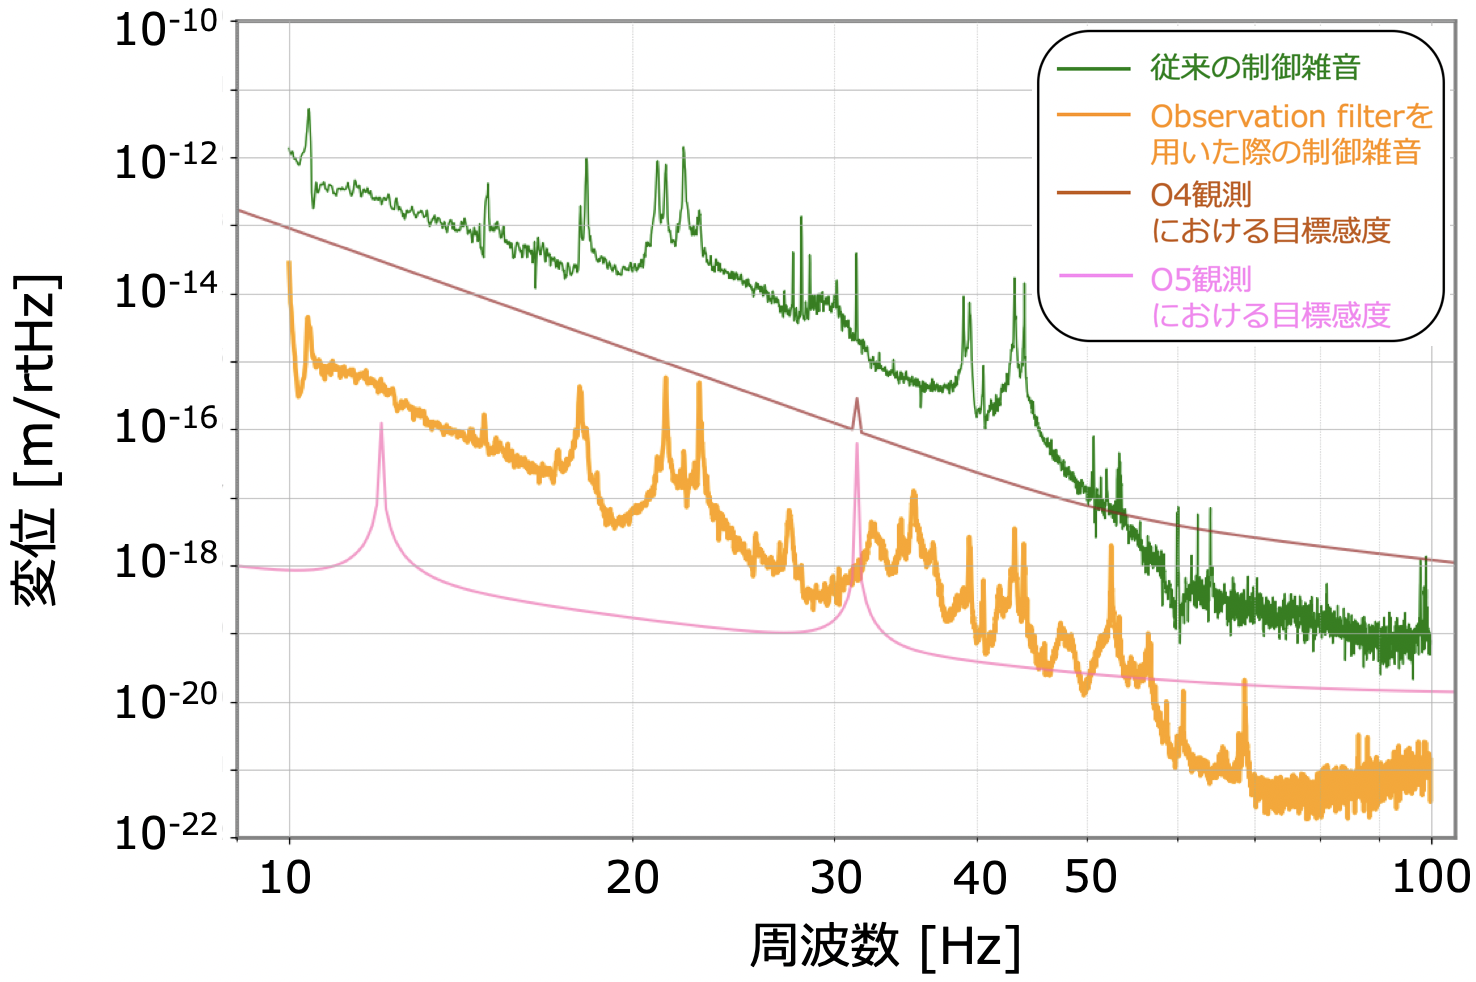
\includegraphics[width=140mm]{fig8_1.png}
\caption[O5観測での目標感度と現在の制御雑音]{O5観測での目標感度と現在の制御雑音. ピンクの線はO5での目標感度である128 Mpcを示している. この感度を達成するためには, $10\sim50$ Hzにおいて制御雑音を$1\sim3$ 桁程度低減する必要がある. そこで, 精密な数値シミュレーションに基づくモーダルダンピングなど, 様々な観点で制御雑音の低減, 感度の向上を目指す.}
\label{fig8.1}
\end{center}
\end{figure}

